\documentclass[11pt,landscape]{article}
\usepackage{multicol}
\usepackage{calc}
\usepackage{ifthen}
\usepackage[landscape]{geometry}
\usepackage{hyperref}
\usepackage{lipsum}  

\ifthenelse{\lengthtest { \paperwidth = 11in}}
	{ \geometry{top=.5in,left=.5in,right=.5in,bottom=.5in} }
	{\ifthenelse{ \lengthtest{ \paperwidth = 297mm}}
		{\geometry{top=1cm,left=1cm,right=1cm,bottom=1cm} }
		{\geometry{top=1cm,left=1cm,right=1cm,bottom=1cm} }
	}

% Turn off header and footer
\pagestyle{empty}
 \usepackage{amsmath}

% Redefine section commands to use less space
\makeatletter
\renewcommand{\section}{\@startsection{section}{1}{0mm}%
                                {-1ex plus -.5ex minus -.2ex}%
                                {0.5ex plus .2ex}%x
                                {\normalfont\large\bfseries}}
\renewcommand{\subsection}{\@startsection{subsection}{2}{0mm}%
                                {-1explus -.5ex minus -.2ex}%
                                {0.5ex plus .2ex}%
                                {\normalfont\normalsize\bfseries}}
\renewcommand{\subsubsection}{\@startsection{subsubsection}{3}{0mm}%
                                {-1ex plus -.5ex minus -.2ex}%
                                {1ex plus .2ex}%
                                {\normalfont\small\bfseries}}
\makeatother

% Define BibTeX command
\def\BibTeX{{\rm B\kern-.05em{\sc i\kern-.025em b}\kern-.08em
    T\kern-.1667em\lower.7ex\hbox{E}\kern-.125emX}}

% Don't print section numbers
\setcounter{secnumdepth}{0}
\usepackage{circuitikz}


\setlength{\parindent}{0pt}
\setlength{\parskip}{0pt plus 0.5ex}
\usepackage{karnaugh-map}


% -----------------------------------------------------------------------

\begin{document}

\raggedright
\footnotesize
\begin{multicols*}{3}


% multicol parameters
% These lengths are set only within the two main columns
%\setlength{\columnseprule}{0.25pt}
\setlength{\premulticols}{1pt}
\setlength{\postmulticols}{1pt}
\setlength{\multicolsep}{1pt}
\setlength{\columnsep}{2pt}

\begin{center}
     \Large{\textbf{CHE374 Final Cheatsheet}}\\
     \small{\textit{Author: QiLin Xue}} \\
\end{center}


\section{Interest}
The compound interest rate is given by
$$F = P\left(1 + \frac{r}{m}\right)^m = P(1+r_\text{eff})$$
where $r$ is the nominal interest rate for 1 period (usually for 1 year), and $m$ is the number of times compounded per period.
\section{Equivalence Factors}
\begin{itemize}
    \item $(F/P,i,N)=(1+i)^N$
    \item $(P/A,i,N) = \frac{(i+1)^N-1}{i(1+i)^N}$
    \item $(P/G,i,N) = \frac{1}{i^2}\left(1-\frac{1+iN}{(1+i)^N}\right)$
    \item $(P/Geom,i,g,N) = \frac{1}{i-g}\left(1-\left(\frac{1+g}{1+i}\right)^N\right)$
\end{itemize}
For geometric,
\begin{equation*}
    P = A(P/Geom,i,g,N)
\end{equation*}
For linear,
\begin{equation*}
    P = G(P/G, i, N).
\end{equation*}
\section{Mortgage}
\begin{itemize}
    \item \textbf{Principal:} The amount of money you borrow to pay for a real property
    \item \textbf{Mortgage rate:} the interest rate charged on the mortgage. Compounding period usually matches frequency of payments
    \item \textbf{Amortization Period:} Time horizon for mortgage payment
    \item \textbf{Term:} Duration of time when the mortgage rate is fixed. When term ends, re-evaluate how much you still owe, then use new interest rate to calculate monthly payment based on time left in amortization period.
\end{itemize}
The net amount owed at end of term is 
\begin{equation*}
    Net = P\left(F/P, i/N, tN\right) - A\left(F/A, i/N, tN\right),
\end{equation*}
where $t$ is the number of years in term and $N$ is the number of payment periods per year. The net monthly payment is 
\begin{equation*}
    A = P\left(A/P, i/N, tN\right),
\end{equation*}
where $t$ is the number of years in amortization (or what is left), and $P$ is the mortgage principal (or what is left).
\section{Bonds}
\begin{itemize}
    \item \textbf{Bond:} a type of loan where the creditor pays a stated amount at specified intervals for a defined period (coupon payments), plus a final amount at a specified date (face value)
    \item \textbf{Coupon rate:} the rate used to calculate coupon payments.
    \item \textbf{Coupon payments:} Regular payment made over the course of a bond's lifetime. Amount determined by coupon rate and frequency of payment.
    \begin{equation*}
        \text{coupon amount} = \text{coupon rate} \times \frac{\text{face value}}{\text{payment frequency}}
    \end{equation*}
    \item \textbf{Yield:} Hypothetical interest rate of a bond given a purchase price. Solved using interpolation.
\end{itemize}
The bond price is given by 
\begin{equation*}
    P = A\left(P/A, i/m, N\right) + F\left(P/F, i/m, N\right),
\end{equation*}
where $i$ is the yield, $m$ is the frequency of coupon payments per time unit, $N$ is the number of periods to maturity ($m\times \text{ time unit}$), and $A$ is the value of coupon payment. Unless otherwise stated, assume all coupons are paid semiannually and the payment is half the coupon rate.
\section{Financial Risk}
The expected rate of return for a company is given by
$$CAPM = E[R_c] = r_f + \beta_c\left(E[R_{MP} - r_f]\right).$$
Let $a$ be the \# of $MP$ shares and $b$ be the \# of risk-free shares. Then,
\begin{align*}
    aP_{MP+} + bP_{r+} = P_{I+} \\ 
    aP_{MP-} + bP_{r-} = P_{I-}
\end{align*}
where
\begin{equation*}
    P_I = aP_{MP} + bP_r.
\end{equation*}
Here, the present market price $P_{MP}$ will take on certain values if it goes up or down. The project/investment price $P_I$ will also take on certain values depending on if market goes up or down. The risk-free rate is $r_f.$ We also have,
\begin{equation*}
    \beta_i = \frac{\sigma_{i,MP}}{\sigma_{MP}^2} = \frac{\rho_{i,MP}\sigma_i}{\sigma_{MP}},
\end{equation*}
where $\sigma_{i,MP}$ is the covariance between $i$th company and market portfolio, $\sigma_{MP}^2$ is the variance of MP, $\rho_{i,MP}$ is the correlation of returns between $i$th company and MP, $\sigma_i$ is volatility of $i$th company, $\sigma_{MP}$ is volatility of MP. If the fair price at $t=0$ is $P_0,$ then the fair price at time $t$ is 
\begin{equation*}
    P_t = P_0 (F/P, CAPM, t).
\end{equation*}
\section{Forward Rates}
\begin{itemize}
    \item Given rates for investments between $t=0$ and $t=t_1$ or $t=t_2$: $t_{0,t_1}$ and $t_{0,t_2},$ respectively. The interest forward rate $t_1$ years from $t=0$ for a duration of $t_2-t_1$ years is 
    \begin{equation*}
        r_{t_1,t_2} = \frac{r_{0,t_2} \cdot t_2 - r_{0,t_1}\cdot t_2}{t_2-t_1}.
    \end{equation*}
\end{itemize}
\section{Example Problems}
$\star$ Suppose an annual yield rate of $7\%,$ (semi-annual compounding), face value \$100. A bond with a coupon rate of $6\%$ maturing in 3 years and 4 months from now is 
\begin{equation*}
    \left(100\cdot \frac{6\%}{2}(P/A,\frac{7\%}{2},7) + 100(P/F,\frac{7\%}{2},7)\right)\left(1+\frac{7\%}{2}\right)^{2/6}
\end{equation*}
$\star$ CAD risk free rate is $3\%.$ US risk free rate is $3\%.$ Current FX is $0.9 US/CAD$, what is the fair FX rate 1 year from now? 
\begin{itemize}
    \item Path 1: Let interest grow on \$1 CAD, gives \$1.03 CAD.
    \item Path 2: Convert \$1 CAD to \$0.9 USD, let interest grow, gives \$0.9225 USD. Then,
\end{itemize}
\begin{equation*}
    FX_1 = \frac{0.9225}{1.03} = 0.896 USD/CAD
\end{equation*}
$\star$ Given house price for \$2,995,000, and we have \$599,000 (enough for 20\% down payment). Mortgage rate is $2\%,$ with a $5$ year term, and a $25$ year amortization period. The monthly interest is 
\begin{equation*}
    (1+2\%/2)^2 = (1+i)^{12} \implies i = 0.16598\%.
\end{equation*} 
The monthly payment is
\begin{equation*}
    2,396,000 = A(P/A,i,300) \implies A = \$10,145.89.
\end{equation*}
$\star$ At the end of term, new mortgage rate is $4\%.$ The amount owed is 
\begin{equation*}
    2,396,000 - 10,145.89(P/A,2\%/12,60) = 2,007,135.
\end{equation*}
Since there are $20$ years left in amortization period, the effective monthly interest is 
\begin{equation*}
    (1+4\%/2)^2 = (1+i)^{12} \implies i =3.967\%,
\end{equation*}
so the annuity is 
\begin{equation*}
    2,007,135 = A(P/A,i,240) \implies A = \$12,128.04.
\end{equation*}
$\star$ Consider mortgage $P$, $N$ total payments at an interest $r$ (based on $N$ compounding periods). If the $m$th payment $(m<n)$ has just been paid, the remaining principal is
\begin{equation*}
    P_m = \frac{P\left[1-(A/P,r,N)(P/A,r,m)\right]}{(P/F,r,m)}
\end{equation*}
$\star$ Consider a 5-year mortgage of \$250,000, with a quoted interest rate of 12.304\% per year with monthly payments. The monthly rate is 
\begin{equation*}
    (1+12.304\%/2)^2 = (1+i)^{12} \implies i = 1\%.
\end{equation*}
$\star$ The principal left on mortgage right after the monthly payment was made at the end of year 2 is \$167,421. The interest charged in the first month of year 3 is given by
\begin{equation*}
    167,421 \times 1\% = 1674.31.
\end{equation*}
$\star$ What would be the break-even penalty fee that you would be willing to pay if we enter into new mortgage contract at the beginning of year 3, with rate quoted at $6.0755\%.$ We have a break-even when monthly payments are the same,
\begin{equation*}
    (1+6.0755\%/2)^2 = (1+i_2)^{12} \implies i_2 = 0.5\%.
\end{equation*}
Then, we can solve for $x_\text{penalty},$
\begin{equation*}
    5561.11 = (167,431.21 + x_\text{penalty})(A/P, 0.5\%, 3\times 12)
\end{equation*}
$\star$ Current market index price is \$105. In the next time period, the market can either go up to \$127, with probability 60\%, or down to \$90. The risk-free rate is 2.2\% per time
period. You have an opportunity to buy a cash flow scenario where if the market goes
up, you will receive \$102.00 and if the market goes down, you will receive \$77.
Determine a fair market price for this scenario. What is the beta for this scenario? We have,
\begin{center}
    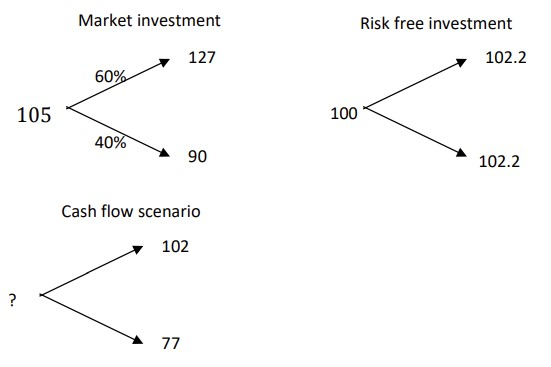
\includegraphics[width=0.8\linewidth]{risk.jpg},
\end{center}
which gives us 
\begin{align*}
    127a + 102.2b = 102 \\ 
    90a +  102.2b = 77,
\end{align*}
which gives $(a,b)=(0.676,0.158).$ The fair price would then be $105a+100b=\$86.79.$ The market expected rate of return is $(127 \cdot 60\% + 90 \cdot 40\%)/105 - 1 = 6.857\%$ and cash flow expected rate of return is $(102\cdot 60\% + 77 \cdot 40\%)/86.79 - 1 = 6.007\%,$ so $$\beta = \frac{6.007\% - 2.2\%}{6.857\% - 2.2\%} = 0.8175.$$ 
$\star$ In the Canadian market, the market index (portfolio) is currently trading at C\$10. If the market goes up, the price is expected to be C\$12 and if the market goes down, the price is expected to be C\$9. The Canadian risk-free rate is 5\% for the period. In the US, the current price of the market index is US\$100. If the market goes up, its price is expected to be US\$110, and if the market goes down, the price is expected to be US\$95. The current exchange rate is 0.80 US$/C$. Assume the Canadian and US markets are 100\% correlated. Determine the US risk-free rate. (Hint: write out the US market payoff in CAD assuming the FX rate one year from now to be FX1 and using no-arbitrage arguments you should be able to solve for FX1, then solve for the interest rate.) We have (no arbitrage),
\begin{align*}
    12a + 1.05b &= 110/FX_1 \\
    9a + 1.05b &= 95/FX_1 \\ 
    10a + b &= 100/0.8, 
\end{align*}
where we converted the USD graph to CAD (hence why we divide by $FX_1$ and $FX_0=0.8$). This gives $a=6.40,$ $b=61.0,$ and $FX_1=0.781.$ Then using the standard conversion (let CAD collect interest, or convert CAD to USD, collect interest, and convert back), we get 
\begin{equation*}
    0.8(1+r_{US}) \times \frac{1}{0.781} = 1.05 \implies r_{US} = 2.5\%.
\end{equation*}
$\star$ Wish to calculate yield rate for a client company, RSG, that is interested in raising
\$10,000,000 through 5 year term bonds with annual coupon payments. Risk-neutral probability of going bankrupt, and thus defaulting on making its future payments is 2\% per coupon payment term (i.e. per year). Assume that the "loss given default" equals 40\% - i.e. if RSG goes bankrupt, no more coupons will be paid and the investors will receive 40\% of the face value of the bond. The risk-free rate is 3\% (annual, effective). You estimate RSG's weighted average cost of
capital to be 7\%. The coupon rate is 5\%. The expected cash flow is,
\begin{center}
    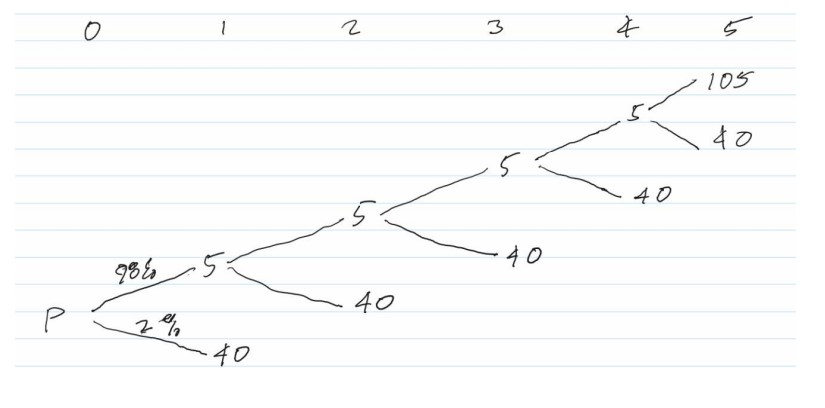
\includegraphics[width=\linewidth]{tree.jpg}
\end{center}
where 
\begin{align*}
    P_0 &= (0.98 \cdot P_1 + 0.02 \cdot 40)/1.03 \\ 
    P_1 &= 5 + (0.98 \cdot P_2 + 0.02 \cdot 40)/1.03 \\
    \cdots & \cdots \\ 
    P_4 &= 5 + (0.98 \cdot 105 + 0.02 \cdot 40)/1.03 = 105.679,
\end{align*}
and work backwards to solve for the price of the bond $P_0=\$103.083$. The yield is therefore given by 
\begin{equation*}
    103.083 = 100 \cdot 5\% (P/A,Y,5) +100(P/F,Y,5).
\end{equation*}
$\star$ Given a bond yield curve where at year 3 the continuously compounded yield is 4.3\% and at year 8 the continuously compounded yield is 5.82\%, at what forward rate should an investor lock into for an investment in a bond, 3 years from now, for 5 years. That is, the investor plans to look into a rate to invest in the bonds for 5 years 3years from now (i.e. a forward rate). We have,
\begin{equation*}
    F_{0,3yr}=P_0e^{r_{3yr}t_3};\quad\quad\quad\quad F_{0,8yr}=P_0e^{r_{8yr}t_8}.
\end{equation*}
Let $r_{3yr,8yr}$ be the forward rate. Then, the following are true:
\begin{align*}
    F_{0,8yr} = F_{0,3yr}e^{r_{3yr,8yr}(t_8-t_3)} \\ 
    P_0e^{r_{8yr}t_8} = P_0 e^{r_{3yr}t_3}e^{r_{3yr,8yr}(t_8-t_3)} \\ 
    r_{3yr,8yr} = \frac{r_{8yr}t_8 - r_{3yr}t_3}{t_8-t_3} = 6.732\%.
\end{align*}
For example, we can compute,
\begin{align*}
    F_8 = 1e^{5.82\% \times 8} \\ 
    F_{3,8} = F_3e^{r_{3,8} \times 5},
\end{align*}
where $F_{3,8}$ is the future value at $t=8$ given present at $t=3.$
\end{multicols*}
\end{document}
